%%%%%%%%%%%%%%%%%%
\subsection[Exploration]{Exploration$^\star$}\label{alg:exploration}
One precondition of the Agents on Mars Scenario is that all agents start with an empty belief base. Each agent does not know about its local and global environment. Of course every agent gets beliefs about its local environment very quickly by receiving percepts from the server. But the agent still does not know about the global environment. For our strategies it is crucial to have as much information about the overall environment as possible. Just think about finding and building the best global zones or pathfinding. So it is important to store somehow information about the map like vertices, edges between vertices, paths and agent positions. In \autoref{alg:map_cartographer} our initial approach with its down- and up-sides is described. After that a basic overview over the Distance-Vector-Algorithm and the impact on our map building approach is given in \autoref{alg:map_dv}. Finally this chapter concludes with a description of the second approach we used and sticked to in \autoref{alg:map_javamap}


%%%%%%%%%%%%%%%%%%
\subsubsection[Cartographer Agent]{Cartographer Agent$^\star$}\label{alg:map_cartographer}
We decided very early in our development process that we do not want to store information which is needed by every agent in each single agent. The intention behind this decision was to reduce the effort in synchronizing and maintaining data between the single agents. Our initial approach was to install one omniscient pseudo agent we called the ``cartographer'' agent. The cartographer agent represented a map and had the only purpose to calculate shortest paths between given vertices and to store vertex and edge information like traversing costs, edges between vertices and vertex values. Every agent told the cartographer agent about its environment related beliefs and the cartographer agent stored these beliefs. Environment related beliefs are illustrated in the listing below:

\begin{lstlisting} [caption={Map exploration related beliefs}, label={lst:dv_exploration_beliefs}]
   visibleEntity(<Vehicle>, <Vertex>, <Team>, <Disabled>).
   position(<Vertex>).
   visibleVertex(<Vertex>, <Team>).
   probedVertex(<Vertex>, <Value>).
   visibleEdge(<VertexA>, <VertexB>).
   surveyedEdge(<VertexA>, <VertexB>, <EdgeCosts>).
\end{lstlisting}

 If an agent needed to know a shortest path, it just queried the cartographer agent and got the shortest path as an answer. Or if an agent needs to know if an vertex was already probed or surveyed, it just queried the cartographer. Shortly after implementing this approach, we encountered two major problems, which both resulted in serious performance issues. One problem was that pathfinding, which was done with the help of the Dijkstra-Algorithm, was executed every time an agent asked for a shortest path. This led to a lot of redundant calculation and processing in the cartographer agent. The second problem was related to communication between agents. To understand the latter problem, one need to know that Jason uses a message box system for communication between agents. This means that every message a sender sends to a receiver is queued in the receivers message inbox. In every Jason lifecycle only one message is processed. Although a Jason lifecycle is a lot shorter than a server lifecycle, still after some execution time the inbox of the cartographer agent was so full, that the processing of messages lagged far behind the receiving of these messages. Both issues resulted in blocked agents, which had been waiting for the response of their queries for rounds.


%%%%%%%%%%%%%%%%%%
\subsubsection[Distance-Vector Routing Protocol]{Distance-Vector Routing-Protocol$^\star$}\label{alg:map_dv}
To tackle the problem of repeating calculations of shortest paths, we used the \emph{Distance-Vector Routing Protocol}(short: DV) \cite{wiki:dvrp}. DV is a routing protocol based on the Bellman-Ford algorithm \cite{wiki:bellman_ford}. DV can be executed on a network of nodes. The basic idea is that each node informs all of its neighbor nodes about its belief base. The informed node then updates its belief base and informs all of its neighbors also and so on. And some point all information is propagated through the whole network and all nodes have a consistent belief base. To adapt this algorithm to our system, we created node agents. A node agent represents one vertex of the scenario map and holds information about this vertex. To make it easier to address node agents, we named node agents like the vertex they represented. A node agent stores all its neighbors in a neighbor-list belief (\texttt{neighbors([<ListOfNeighbors>])}) and all available paths to other vertices as path beliefs (\texttt{path(<Destination>, <NextHop>, <Hops>, <CostToNextHop>)}). With regard to exploration and zoning we decided that an node agent also has to store the probed value of the vertex, and if it was already probed or surveyed.

\begin{samepage}
For a better illustration see the following example of the belief base of the node agent \texttt{v1}:
\begin{itemize}
  \item \texttt{neighbors([v2, v3]).}
  \item \texttt{probed(true).}
  \item \texttt{probedValue(7).}
  \item \texttt{surveyed(true).}
  \item \texttt{path(v1, v1, 0, 0).}
  \item \texttt{path(v2, v2, 1, 3).}
  \item \texttt{path(v10, v2, 4, 3).}
  \item \texttt{path(v8, v3, 3, 2).}
\end{itemize}
\end{samepage}

A query for a shortest path would look like this:
\begin{lstlisting}[caption={Query for shortest path from \texttt{v1} to \texttt{v8}}, label={lst:dv_shortestPath_query}]
  .send(v1, askOne, path(v8, NextHop, _, CostToNextHop)).
\end{lstlisting}
After looking up the belief in its belief base the node agent would unify the parameter \texttt{NextHop} with \texttt{v3} and CostToNextHop with \texttt{2} and response to the querying agent.

So now we know what information a node agent holds and how it can be addressed. But how does it get its data? How can we assure that it is always the best path we get if we query the node agent? Here the Distance-Vector Routing Protocol comes into play. When an real agent, unlike the virtual node agents, stands on a vertex it gets a lot of beliefs from the server, see \autoref{lst:dv_exploration_beliefs}. The \texttt{visibleEdge(<VertexA>, <VertexB>)} belief and the \texttt{surveyedEdge(<VertexA>, <VertexB>, <EdgeCost>)} belief are showing all connected vertices and hence all neighbors tuples. The real agent informs the respective node agent about its neighbor, who then updates its neighbor-list and adds or updates the path to this neighbor.

\begin{lstlisting}[caption={Real agent informs node agent about its neighbor}, label={lst:dv_neighbor_inform}]
  RealAgent: 
  +visibleEdge(VertexA, VertexB) <- 
    .send(VertexA, tell, neighbor(VertexB, 10)).
  
  +surveyedEdge(VertexA, VertexB, Value) <- 
    .send(VertexA, tell, neighbor(VertexB, Value)).
    
  NodeAgent:
  +neighbor(Vertex, Value):
    path(Vertex, Vertex, Hops, Costs)
    & Value < Costs
    <- 
    -path(Vertex, Vertex, Hops, Costs);
    +path(Vertex, Vertex, 1, Value).
        
  +neighbor(Vertex, Value):
    neighbors(List)
    & <Vertex not in List>
    <-
    .abolish(neighbors(_)); 
    +neighbors([Vertex|List]);
    +path(Vertex, Vertex, 1, Value).  
\end{lstlisting}

After updating its belief base the node agent informs all its neighbors about the changes. And these neighbors also inform their neighbors and so on. At some point the belief base of each node agent is consistent and no further broadcasting is needed. \autoref{fig:dv} demonstrates the procedure for a small set of four neighbor nodes.

\begin{figure}
  \centering
  \subcaptionbox{caption0 \label{fig:dv_0}}[.40\linewidth]{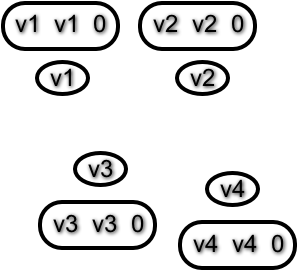
\includegraphics[width=.40\linewidth]{images/dv0.png}}
  \subcaptionbox{caption1 \label{fig:dv_1}}[.40\linewidth]{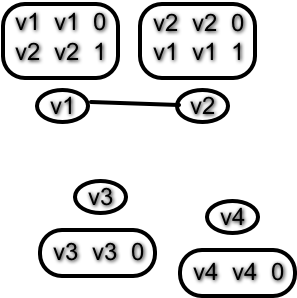
\includegraphics[width=.40\linewidth]{images/dv1.png}}
   \subcaptionbox{caption2 \label{fig:dv_2}}[.40\linewidth]{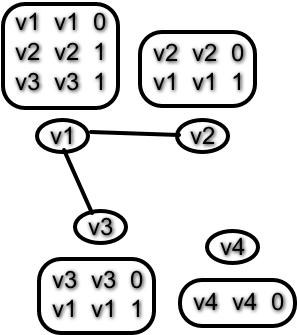
\includegraphics[width=.40\linewidth]{images/dv2.png}}
   \subcaptionbox{caption3 \label{fig:dv_3}}[.40\linewidth]{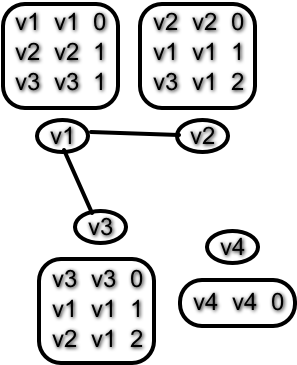
\includegraphics[width=.40\linewidth]{images/dv3.png}}
   \subcaptionbox{caption4 \label{fig:dv_4}}[.40\linewidth]{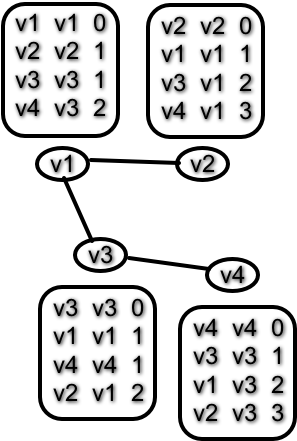
\includegraphics[width=.40\linewidth]{images/dv4.png}}
   \subcaptionbox{caption5 \label{fig:dv_5}}[.40\linewidth]{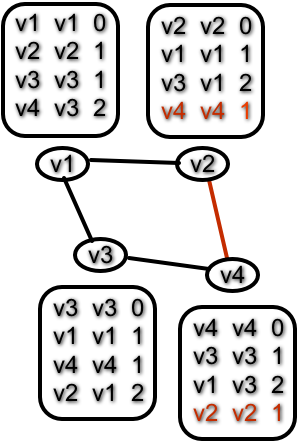
\includegraphics[width=.40\linewidth]{images/dv5.png}}
                 
  \caption{Executing the Distance-Vector Routing Protocol algorithm as described in \autoref{alg:map_dv} on a small network of four nodes. Each node has a table attached, containing all accessible nodes. The first parameter is the destination node, the second one is the node to pass through and the third parameter shows the overall distance to the destination.}
  \label{fig:dv}
\end{figure}

What is it? How is it used in our context? What are advantages we gain from it? What is problematic (speed loss)?

%%%%%%%%%%%%%%%%%%
\subsubsection[JavaMap]{JavaMap$^\star$}\label{alg:map_javamap}